\documentclass[11pt]{article} 
\usepackage[utf8]{inputenc}

\usepackage{deauthor,times}
\usepackage{graphicx}
\usepackage{hyperref}
\usepackage{amsfonts,amsmath}
\usepackage{enumitem}
\usepackage{xspace} 
\usepackage{xcolor}

\newcommand*{\rf}{\textsf{Ranking Facts}\xspace}
\newcommand*{\eg}{e.g.,\xspace}
\newcommand*{\ie}{i.e.,\xspace}
\newcommand{\etal}{et al.\xspace}

\newcommand{\fairprep}{\stt{FairPrep}\xspace}
\newcommand{\aif}{\stt{AIF360}\xspace}
\newcommand{\sklearn}{\stt{scikit-learn}\xspace}
\newcommand{\pandas}{\stt{pandas}\xspace}
\newcommand{\mlinspect}{\stt{mlinspect}\xspace}
\newcommand{\deequ}{\stt{Deequ}\xspace}


\newcommand{\adult}{\texttt{adult}\xspace}
\newcommand{\german}{\texttt{germancredit}\xspace}
\newcommand{\propublica}{\texttt{propublica}\xspace}
\newcommand{\ricci}{\texttt{ricci}\xspace}


\newcommand{\header}[1]{\vspace{1mm}\noindent\textbf{#1}.}
\newcommand{\headerl}[1]{\vspace{1mm}\noindent\textit{#1}.}

\newcommand{\rev}[1]{#1}
\newcommand{\revtammo}[1]{#1}

\newcommand{\todo}[1]{\textcolor{purple}{TODO: #1}}

\usepackage{tikz}
\newcommand*\circled[1]{\tikz[baseline=(char.base)]{\node[shape=circle,fill=black,draw,inner sep=0.6pt] (char) {\textcolor{white}{\footnotesize \textbf{#1}}};}}

\newcommand{\julia}[1]{\textcolor{teal}{[Julia: #1]}}
\newcommand{\sebastian}[1]{\textcolor{blue}{[Julia: #1]}}

\newcommand{\shref}[2]{{\footnotesize\href{#1}{#2}}}
\newcommand{\surl}[1]{{\footnotesize\url{#1}}}
\newcommand{\stt}[1]{{\footnotesize\texttt{#1}}}

\usepackage[T1]{fontenc}
\usepackage{beramono}
\usepackage{listings}
\usepackage{xcolor}

\definecolor{dkgreen}{rgb}{0,0.6,0}
\definecolor{gray}{rgb}{0.5,0.5,0.5}
\definecolor{mauve}{rgb}{0.58,0,0.82}

\lstdefinestyle{myScalastyle}{
  frame=tb,
  language=scala,
  aboveskip=3mm,
  belowskip=3mm,
  showstringspaces=false,
  columns=flexible,
  basicstyle={\scriptsize\ttfamily},
  numbers=none,
  numberstyle=\tiny\color{gray},
  keywordstyle=\color{blue},
  commentstyle=\color{dkgreen},
  stringstyle=\color{mauve},
  frame=single,
  breaklines=true,
  breakatwhitespace=true,
  tabsize=3,
}

\begin{document}

\title{Taming Technical Bias in Machine Learning Pipelines
\footnote{This work was supported in part by NSF Grants No. 1926250, 1934464, and 1922658, and by Ahold Delhaize. All content represents the opinion of the authors, which is not necessarily shared or endorsed by their respective employers and/or sponsors.}}

\author{
Sebastian Schelter\\
University of Amsterdam \& Ahold Delhaize\\
Amsterdam, The Netherlands \\
s.schelter@uva.nl
\and
 Julia Stoyanovich \\
New York University \\
New York, NY, USA \\
stoyanovich@nyu.edu}

\maketitle

\begin{abstract}
Machine Learning (ML) is commonly used to automate decisions in domains as varied as credit and lending,  medical diagnosis, and  hiring.  These decisions are consequential, imploring us to carefully balance the benefits of efficiency with the potential risks.   Much of the conversation about the risks centers around bias --- a term that is used by the technical community ever more frequently but that is still poorly understood. 
In this paper we focus on technical bias --- a type of bias that has so far received limited attention and that the data engineering community is well-equipped to address. We discuss dimensions of technical bias that can arise through the ML lifecycle, particularly when it's due to preprocessing decisions or post-deployment issues.  We present results of our recent work, and discuss future research directions. Our over-all goal is to support the development of systems that  expose the knobs of responsibility to data scientists, allowing them to detect instances of technical bias and to mitigate it when possible.
\end{abstract}

\section{Introduction}
\label{sec:intro}

Machine Learning (ML) is increasingly used to automate  decisions that impact people's lives, in domains as varied as credit and lending,  medical diagnosis, and  hiring. The risks and opportunities arising from the wide-spread use of predictive analytics are garnering much attention from policy makers, scientists, and the media.  Much of this conversation centers around \emph{bias} --- a term that is used by the technical community ever more frequently but that is still poorly understood. 

In their seminal 1996 paper, Friedman and Nissenbaum identified three types of bias that can arise in computer systems: pre-existing, technical, and emergent ~\cite{DBLP:journals/tois/FriedmanN96}.    We briefly discuss these in turn, see Stoyanovich~\etal~\cite{DBLP:journals/pvldb/StoyanovichHJ20} for a more comprehensive  overview.

\begin{itemize}[leftmargin=*]
\item \emph{Pre-existing  bias} has its origins in society.  In ML applications, this type of bias often exhibits itself in the input data; detecting and mitigating it is the subject of much research under the heading of algorithmic fairness~\cite{DBLP:journals/cacm/ChouldechovaR20}. Importantly, the presence or absence of pre-existing bias cannot be scientifically verified, but rather is postulated based on a belief system~\cite{DBLP:journals/corr/FriedlerSV16,DBLP:conf/fat/HeidariLGK19}. Consequently, the effectiveness --- or even the validity --- of a technical attempt to mitigate pre-existing bias is predicated on that belief system.

\item \emph{Technical bias} arises due to the operation of the technical system itself, and can amplify pre-existing bias.  The bad news is that, as we argue in the remainder of this paper, the risks of introducing technical bias in ML pipelines abound. The good news is that, unlike with pre-existing bias, there is no ambiguity about whether a technical fix should be attempted: if technical systems we develop are introducing bias, then we should be able to instrument these systems to measure it and understand its cause. It may then be possible to mitigate this bias and to check whether the mitigation was effective.

\item \emph{Emergent bias}   arises in the context of use of the technical system. In Web ranking and recommendation in e-commerce, a prominent example is ``rich-get-richer'': searchers tend to trust the systems to indeed show them the most suitable items at the top positions, which in turn shapes a searcher's idea of a satisfactory answer.

\end{itemize}

In this paper, we focus on technical bias,  --- a type of bias that has so far received limited attention, particularly when it's due to preprocessing decisions or post-deployment issues, and that the data engineering community is well-equipped to address.  Our over-all goal is to support the development of systems that \emph{expose the knobs of responsibility to data scientists}, allowing them to detect instances of technical bias, and to mitigate it when possible.


\header{Running example} We illustrate the need for taming technical bias with an example from the medical domain. Consider a data scientist who implements a Python pipeline that takes demographic and clinical history data as input, and trains a classifier to identify patients at risk for serious complications. Further, assume that the data scientist is under a legal obligation to ensure that the resulting ML model works equally well for patients across different gender and age groups.  This obligation is operationalized as an intersectional fairness criterion, requiring equal false negatives rates for groups of patients identified by a combination of gender and age group. 

Consider Ann, a data scientist who is developing this classifier. Following her company's best practices, Ann will start by splitting her dataset into training, validation, and test sets. Ann will then use \pandas, \sklearn~\cite{Pedregosa2011}, and their accompanying data transformers to explore the data and implement data preprocessing, model selection, tuning, and validation. Ann starts preprocessing by computing value distributions and correlations for the features in her dataset, and by identifying missing values. She will fill these in using a default interpolation method in scikit-learn, replacing missing values with the mode value for that feature.  Finally, following the accepted best practices at her company, Ann implements model selection and hyperparameter tuning. As a result of this step, Ann will select a classifier that shows acceptable performance according to her company's standard metrics: it has sufficient accuracy, while also exhibiting sufficiently low variance. 
When Ann considers the accuracy of her classifier closely, she observes a disparity: accuracy is lower for middle-aged women. Ann is now faced with the challenge of figuring out why this is the case, whether any of her technical choices during pipeline construction contributed to this model bias, and what she can do to mitigate this effect. We will revisit this example, and also discuss issues that may arise after the model is deployed, in the remainder of this paper.

\header{Roadmap} The rest of this paper is organized as follows.  In Section~\ref{sec:dim}, we
outline the dimensions of technical bias as they relate to two lifecycle views of ML applications: the data lifecycle and the lifecycle of design, development, deployment, and use.  Then, in Section~\ref{sec:fairprep} we present our recent work on helping data scientists responsibly develop ML pipelines, and validate them post-deployment.  We conclude in Section~\ref{sec:conc} with directions for future research.

\section{Dimensions of Technical Bias}
\label{sec:dim}

There are many different ways in which Ann (or her colleagues who deploy her model) could accidentally introduce technical bias.  Some of these relate to the view of ML model development through the lens of the \emph{data lifecycle}. As argued in Stoyanovich~\etal~\cite{DBLP:journals/pvldb/StoyanovichHJ20}, responsibility concerns, and important decision points, arise in data sharing, annotation, acquisition, curation, cleaning, and integration.   Thus, opportunities for improving data quality and representativeness, controlling for bias, and allowing humans to oversee the process, are missed if we do not consider these earlier data lifecycle stages.  We discuss these dimensions of technical bias in Section~\ref{sec:bias-development}.  Additional challenges, and opportunities to introduce technical bias, arise after a model is deployed.  We discuss these in Section~\ref{sec:bias-deployment}.

Note that, in contrast to Bower \etal~\cite{DBLP:journals/corr/BowerKNSVV17} and Dwork \etal~\cite{DBLP:conf/forc/DworkIJ20}, who study fairness in ML pipelines in which multiple models are composed, we focus on complex --- and typical --- pipelines in which bias may arise due to the composition of data preprocessing steps, or to data distribution shifts past deployment.  

\subsection{Model Development Stage}
\label{sec:bias-development}

There are several subtle ways in which data scientists can accidentally introduce data-related bias into their models during the development stage.  Our discussion in this section is inspired by the early influential work by Barocas and Selbst~\cite{Barocas2016}, and by Lehr and Ohm~\cite{LehrOhm2017}, who highlighted the issues that we will make more concrete.

\header{Data cleaning}
Methods for missing value imputation that are based on incorrect assumptions about whether data is missing at random may distort protected group proportions. Consider a form that gives patients a binary choice of gender and also allows to leave gender unspecified. Suppose that about half of the users identify as men and half as women, but that women are more likely to omit gender.  Then, if mode imputation (replacing a missing value with the most frequent value for the feature, a common choice in \sklearn) is used, then all (predominantly female) unspecified gender values will be set to male.  More generally, multi-class classification for missing value imputation typically only uses the most frequent classes as target variables~\cite{Biessmann2018}, leading to a distortion for small population groups, because membership in these groups will never be imputed. Next, suppose that some individuals identify as non-binary.  Because the system only supports male, female, and unspecified as options, these individuals will leave gender unspecified.  If mode imputation is used, then their gender will be set to male.  A more sophisticated imputation method will still use values from the active domain of the feature, setting the missing values of gender to either male or female.  This example illustrates that  bias can arise from an incomplete or incorrect choice of data representation.
 
Finally, consider a form that has home address as a field.  A homeless person will leave this value unspecified, and it is incorrect to attempt to impute it. While dealing with \stt{null} values is known to be difficult and is already considered among the issues in data cleaning, the needs of responsible data management introduce new problems. Further, data quality issues often disproportionately affect members of historically disadvantaged groups~\cite{kappelhof2017}, and so we risk compounding technical bias due to data representation with pre-existing bias. 

\header{Data filtering} Selections and joins can arbitrarily change the proportion of protected groups (\eg for certain age groups) even if they do not directly use the sensitive attribute (\eg age) as part of the predicate or of the join key.  This change in proportion may be unintended and is important to detect, particularly when this happens during one of many preprocessing steps in the ML pipeline. During model development, Ann might have filtered the data by zip code or county to get a sample that is easier to work with. Demographic attributes such as age and income are highly correlated with places of residency, so such a seemingly innocent filtering operation might have heavily biased the data.

Another potential source of technical bias is the increasingly common usage of pre-trained word embeddings. For example, Ann's code might replace a textual name feature with the corresponding vector from a word embedding that is missing for rare, non-western names (due to lack of data representation in the training corpus). If we then filter out records for which no embedding was found, we may disproportionately remove individuals from specific ethnic groups.  

\header{Unsound experimentation} 
Design and evaluation of ML models is a difficult and tedious undertaking and requires data scientists to strictly follow a set of best practices. During this process, it is unfortunately easy to make subtle mistakes that can heavily impact the quality of the resulting model. In previous research, we found that even expert users violate such best practices in highly cited studies~\cite{DBLP:conf/edbt/SchelterHKS20}. Common mistakes include hyperparameter selection on the test set instead of the validation set, lack of hyperparameter tuning for baseline learners, lack of proper feature normalisation, or ignoring problematic data subsets during training.  

While unsound experimentation is a general issue,  ignoring problematic data subsets can specifically affect performance for minority and underrepresented groups, because their data might be prone to data quality issues, as we already discussed under \emph{data filtering} above.

\subsection{Model Deployment Stage}
\label{sec:bias-deployment}

After the design of a model is finished, the model is deployed into production and produces predictions on unseen data. We outline a set of circumstances which can introduce technical bias at this stage.

\header{Data errors introduced through integration} In modern information infrastructures, data is stored in different  environments (\eg in relational databases, in ‘data lakes’ on distributed file systems, or behind REST APIs), and it comes in many different formats. Many such data sources do not support integrity constraints and data quality checks, and often there is not even an accompanying schema available as the data is consumed in a ‘schema-on-read’ manner, where a particular application takes care of the interpretation. Additionally, there is a growing demand for applications consuming semi-structured data such as text, videos, and images.  Due to these circumstances, every real world ML application has to integrate data from multiple sources, and errors in the data sources or during  integration may lead to errors in downstream ML models that consume the data. 

In our running example in Section~\ref{sec:intro}, it may be the case that  patient data is integrated from data sources of different healthcare providers. If one of these providers accidentally changes their schema, or introduces bugs in their data generation procedure, this may negatively impact the predictions for the corresponding patients when their data is used as input to Ann's model. 

\header{Distribution shifts} The maintenance of ML applications remains challenging~\cite{Polyzotis2018}, due in large part to unexpected shifts in the distribution of serving data. These shifts originate from changes in the data generating process in the real world, and the problem is exacerbated in situations where different parties are involved in the provision of the data and the training of the model. Many engineering teams, especially in smaller companies, lack ML expert knowledge, and therefore often outsource the training of ML models to data science specialists or cloud ML services. In such cases, the engineering team provides the input data and retrieves predictions, but might not be familiar with details of the model. While ML experts have specialized knowledge to debug models and predictions in such cases~\cite{lipton2018detecting}, there is a lack of automated methods for non-ML expert users to decide whether they can rely on the predictions of an ML model on unseen data. In Ann's case, her final deployed model might work well until new regulations for health care providers change the shape and contents of the patient data that they produce. If her model is not retrained on proper data, its prediction quality may quickly deteriorate.


In the following section we will introduce three  software libraries that we developed in recent research to help data scientists like Ann in detecting and mitigating technical bias during model development and deployment.

% !TEX root = main.tex

\section{Taming Technical Bias during Model Development and Deployment}
\label{sec:fairprep}

In Schelter~\etal~\cite{DBLP:conf/edbt/SchelterHKS20} we described \fairprep, a design and evaluation framework for fairness-enhancing interventions in machine learning pipelines that treats data as a first-class citizen.  The framework implements a modular data lifecycle, enables re-use of existing implementations of fairness metrics and interventions, and integration of custom feature transformations and data cleaning operations from real world use cases. \fairprep pursues the following goals: $(i)$~Expose a developer-centered design throughout the lifecycle, which allows for low effort customization and composition of the framework's components; $(ii)$~Surface discrimination and due process concerns, including disparate error rates, failure of a model to fit the data, and failure of a model to generalize. $(iii)$~Follow software engineering and machine learning best practices to reduce the technical debt of incorporating fairness-enhancing interventions into an already complex development and evaluation scenario~\cite{Schelter2018c,Sculley2015}.  


\begin{figure*}[t!]
  \centering
  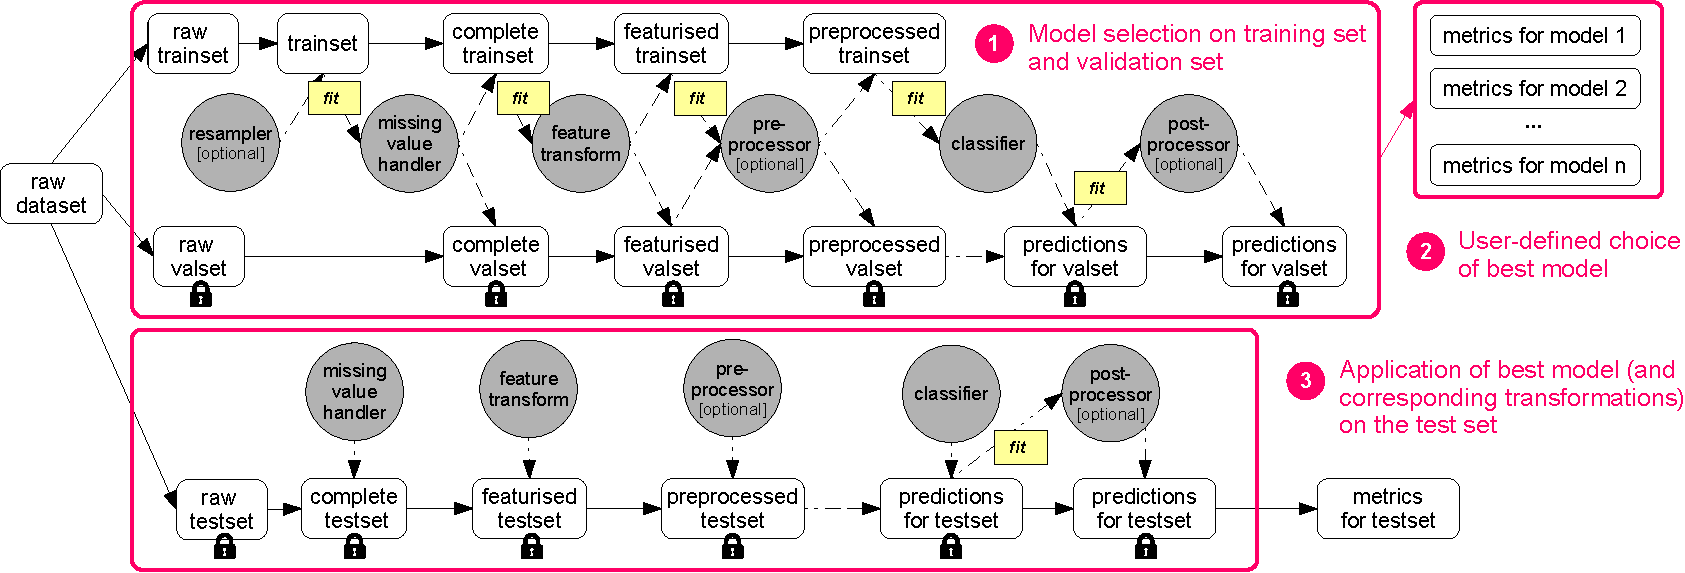
\includegraphics[scale=0.5]{figs/bigpicture-crop}  
  \caption{Data life cycle in \fairprep, designed to enforce isolation of  test data, and to allow for customization through user-provided implementations of different components. An evaluation run consists of three different phases: (1)~Learn different models, and their corresponding data transformations, on the training set; (2)~Compute performance / accuracy-related metrics of the model on the validation set, and allow the user to select the `best' model according to their setup; (3)~Compute predictions and metrics for the user-selected best model on the held-out test set.}
  \label{fig:bigpicture}
\end{figure*}

Figure~\ref{fig:bigpicture} summarizes the architecture of \fairprep, which is based on three main principles: 

\begin{enumerate}
\item Data isolation: to avoid target leakage, user code should only interact with the training set, and never be able to access the held-out test set. 

\item Componentization: different data transformations and learning operations should be implementable as single, exchangeable standalone components; the framework should expose simple interfaces to users, supporting low effort customization. 

\item Explicit modeling of the data lifecycle: the framework defines an explicit, standardized data lifecycle that applies a sequence of data transformations and model training in a predefined order. 
\end{enumerate}

\fairprep  currently focuses on data cleaning, including different methods for data imputation, and model selection and validation, including hyperparameter tuning, and can be extended to accommodate earlier lifecycle stages, such as data acquisition, integration, and curation.   Schelter~\etal~\cite{DBLP:conf/edbt/SchelterHKS20} measured the impact of sound best practices, such as hyperparameter tuning and feature scaling, on the fairness and accuracy of the resulting classifiers, and also showcased how \fairprep enables the inclusion of incomplete data into studies and helps analyze the effects.  

If Ann wants to ensure that she follows sound experimentation practices during model development, she can use the \fairprep library as a runtime platform for experiments, for example to compute various fairness related metrics for the predictions of her classifier. Furthermore, she can leverage the component architecture of \fairprep to evaluate different missing value imputation techniques and fairness enhancing interventions to see whether these help with mitigating the low accuracy that she encountered in her model for the predictions for middle-aged women, as discussed in our running example in Section~\ref{sec:intro}.

\header{Source code} A prototype implementation of FairPrep is available at \surl{https://github.com/DataResponsibly/FairPrep}.

% !TEX root = main.tex
\subsection{Detecting Data Distribution Bugs Introduced in Preprocessing}
\label{sec:mlinspect}

In our recent work on the \textit{mlinspect} library~\cite{grafberger2021mlinspect}, we focus on helping data scientists diagnose and mitigate problems to which we collectively refer as \emph{data distribution bugs}. These types of bugs are often introduced during preprocessing, for reasons we outlined in Section~\ref{sec:dim}.  For example, preprocessing operations that involve filters or joins can heavily change the distribution of different groups in the training data~\cite{fairdags}, and missing value imputation can also introduce skew~\cite{schelter2019fairprep}.  Recent ML fairness research, which mostly focuses on the use of learning algorithms on static datasets~\cite{DBLP:journals/cacm/ChouldechovaR20} is therefore insufficient, because it cannot address such technical bias originating from the data preparation stage. In addition, we should detect and mitigate such bias as close to its source as possible.

Unfortunately, such data distribution issues are difficult to catch. In part, this is because different pipeline steps are implemented using different libraries and abstractions, and the data representation often changes from relational data to matrices during data preparation. Further, preprocessing in the data science ecosystem~\cite{dataScienceLookingGlass} often combines relational operations on tabular data with  \textit{estimator/transformer pipelines},\footnote{\url{https://scikit-learn.org/stable/modules/compose.html}} a composable and nestable abstraction for combining operations on array data, which originates from \stt{scikit-learn}~\cite{Pedregosa2011} and has been adopted by popular libraries like \stt{SparkML}~\cite{meng2016mllib} and \stt{Tensorflow Transform}. In such cases, tracing problematic  featurised entries back to the pipeline's initial human-readable input is tedious work.  Finally, complex estimator/transformer pipelines are hard to inspect because they often result in nested function calls not obvious to the data scientist.

Due to time pressure in their day-to-day activities, most data scientists will not invest the necessary time and effort to manually instrument their code or insert logging statements for tracing as required by model management systems~\cite{Vartak2018,zaharia2018accelerating}.  This calls for the development of tools that support \emph{automated inspection of ML pipelines}, similar to the inspections used by modern IDEs to highlight potentially problematic parts of a program, such as the use of deprecated code or problematic library functions calls. Once data scientists are pointed to such issues, they can use data debuggers like \stt{Dagger}~\cite{maddendagger} to drill down into the specific intermediate pipeline outputs and explore the root cause of the issue. Furthermore, to be most beneficial, automated inspections need to work with code natively written with popular ML library abstractions. 

\header{Lightweight inspection with \mlinspect} To enable lightweight pipeline inspection, we designed and implemented \mlinspect~\cite{grafberger2021mlinspect}, a library that helps data scientists automatically detect data distribution issues in their ML pipelines, such as the accidental introduction of statistical bias, and provides linting for best practices. The \mlinspect library extracts logical query plans, modeled as directed acyclic graphs (DAGs) of preprocessing operators from ML pipelines that use  popular libraries like \pandas and \sklearn, and combine relational operations and estimator/transformer pipelines. These plans are then used to automatically instrument the code and trace the impact of operators on properties like the distribution of sensitive groups in the data. 

Importantly, \mlinspect implements a library-independent interface to propagate annotations such as the lineage of tuples across operators from different libraries, and introduces only constant overhead per tuple flowing through the DAG. Thereby, the library offers a general runtime for pipeline inspection, and allows us to integrate many issue detection techniques that previously required custom code, such as automated model validation on data slices~\cite{SliceFinder}, the identification of distortions with respect to protected group membership in the training data~\cite{fairdags}, or automated sanity checking for ML datasets~\cite{hynes2017data}.

\begin{figure*}[t!]
  \centering
  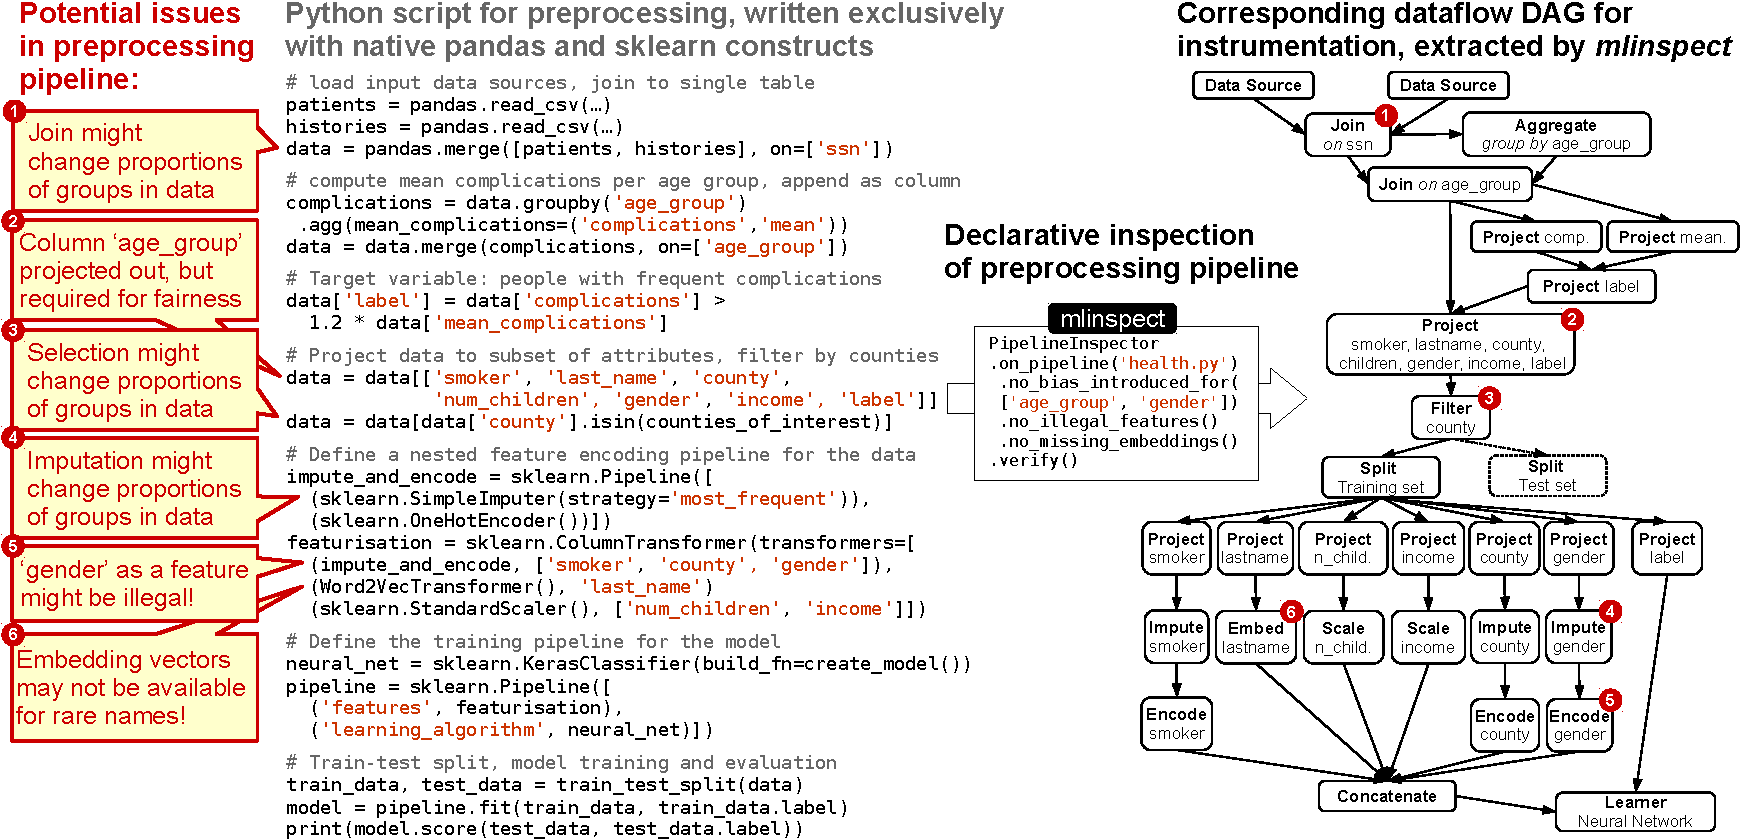
\includegraphics[width=\textwidth]{figs/example-crop}
  \caption{ML pipeline for our running example that predicts which patients are at a higher risk of serious complications, under the requirement to achieve comparable false negative rates across intersectional groups by gender and age group.  On the left, we highlight potential issues identified by \mlinspect. On the right, we show the corresponding dataflow graph, extracted to instrument the code and pinpoint the issues.}
  \label{fig:example}
\end{figure*}

\header{Identifying data distribution bugs in our running example} Figure~\ref{fig:example} shows a  preprocessing pipeline and potential data distribution bugs for our running example from Section~\ref{sec:intro}. The pipeline first reads two CSV files, which contain patient demographics and their clinical histories, respectively. Next, these dataframes are joined on the \stt{ssn} column. This join may introduce a data distribution bug (as indicated by issue \circled{1}) if a large percentage of the records of some combination of gender and age group do not have matching entries in the clinical history dataset. Next, the pipeline computes the average number of complications per age group and adds the binary target label to the dataset,  indicating which patients had a higher than average number of complications compared to their age group. The data is then projected to a subset of the attributes, to be used by the classification model. This leads to the second issue \circled{2} in the pipeline: the data scientist needs to ensure that the model achieves comparable accuracy across different age groups, but the age group attribute is projected out here, making it difficult to catch data distribution bugs later in the pipeline. The data scientist additionally filters the data to only contain records from patients within a given set of counties.  This may  lead to issue \circled{3}: a data distribution bug may be introduced if populations of different counties systematically differ in age.

Next, the pipeline creates a feature matrix from the dataset by applying common feature encoders with  \shref{https://scikit-learn.org/stable/modules/generated/sklearn.compose.ColumnTransformer.html}{\texttt{ColumnTransformer}} from \sklearn, before training a neural network on the features.   For the categorical attributes \stt{smoker}, \stt{county}, and \stt{gender}, the pipeline imputes missing values with mode imputation (using the most frequent attribute value), and subsequently creates one-hot-encoded vectors from the data. The \stt{last\_name} is replaced with a corresponding vector from a pretrained word embedding, and the numerical attributes \stt{num\_children} and \stt{income} are normalized. This feature encoding part of the pipeline introduces several potential issues: \circled{4} the imputation of missing values for the categorical attributes may introduce statistical bias, as it may associate records with a missing value in the gender attribute with the majority gender in the dataset; \circled{5} depending on the legal context (\ie if the disparate treatment doctrine is enforced), it may be forbidden to use \stt{gender}  as an input to the classifier; \circled{6} we may not have vectors for rare non-western names in the word embedding, which may in turn lead to lower model accuracy for such records. As illustrated by this example, preprocessing can give rise to subtle data distribution bugs that are difficult to identify manually, motivating the development of automatic inspection libraries such as \mlinspect, which will hint the data scientist towards these issues.

\header{Source code} A prototype implementation of \mlinspect, together with a computational notebook that shows how \mlinspect can be used to address the issues outlined in the ML pipeline in Figure~\ref{fig:example},  is available at \surl{https://github.com/stefan-grafberger/mlinspect}.


% !TEX root = main.tex
\subsection{Validating Serving Data with Data Unit Tests}
\label{sec:validate}

Machine learning (ML) techniques are very sensitive to their input data, as the deployed models rely on strong statistical assumptions about their inputs~\cite{sculley2015hidden}, and subtle errors introduced by changes in the data distribution can be hard to detect~\cite{polyzotis2017data}. At the same time, there is ample evidence that the volume of data available for training is often a decisive factor for a model’s performance~\cite{halevy2009unreasonable}.  How errors in the data affect performance, and fairness of deployed machine learning models is an open and pressing research question, especially in cases where the data describing protected groups has a higher likelihood of containing errors or missing values~\cite{DBLP:conf/edbt/SchelterHKS20}.

\header{Unit tests for data with \deequ} As discussed in Section~\ref{sec:bias-deployment}, accidental errors during data integration can heavily impact the prediction quality of downstream ML models. We therefore postulate that there is a pressing need for increased automation of data validation.   To respond to this need,
Schelter~\etal~\cite{schelter2018automating} presented \deequ, a data unit testing library. The library centers around the vision  that users should be able to write ‘unit-tests’ for data, analogous to established testing practices in software engineering, and is built on the following principles: 

\begin{enumerate}
    \item Declarativeness:  allowing data scientist to spend time on thinking about \emph{what} their data should look like, and not about \emph{how} to implement the quality checks.   \deequ offers a declarative API that allows users to define checks on their data by composing a variety of available constraints. 
    \item Flexibility: allowing users to leverage external data and custom code for validation (\eg call a REST service for some data and write a complex function that compares the result to some statistic computed on the data).  
    \item Continuous integration: explicitly supporting the incremental computation of quality metrics on growing datasets~\cite{schelter2019differential}, and allowing users to run anomaly detection algorithms on the resulting historical time series of quality metrics.
    \item Scalability: scaling seamlessly to large datasets, by translating the  data metrics computations to aggregation queries, which can be efficiently executed at scale with a distributed dataflow engine such as \stt{Apache Spark}~\cite{zaharia2012resilient}.
\end{enumerate}

\header{Unit testing serving data in our running example} A prime use case of \deequ in ML deployments is to test new data to be sent to the model for prediction. When Ann deploys her model for real world usage, she wants to make sure that it will only consume well-formed data. She can use \deequ to write down her assumptions about the data as a declarative data unit test, and have this test integrated into the pipeline that feeds data to the deployed model. If any  assumptions are violated, the pipeline will stop processing, the data will be quarantined, and a data engineer will be prompted to investigate the root cause of the failure.

Listing~\ref{lst:deequ} shows what  a data unit test may look like. We precompute certain expected statistics for the data such as the number patients to predict for, the valid age groups, and expected distributions by gender and age group. Next, we write down our assumptions about the data, similar to integrity constraints in relational databases. We declare the following checks: we assume that the size of the data corresponds to the expected number of patients, we expect social security numbers (the \stt{ssn} attribute) to be unique, and we expect no missing values for the \stt{lastname}, \stt{county}, and \stt{age\_group} attributes. We furthermore assume that the values of the \stt{smoker} attribute are Boolean, while in the \stt{num\_children} attribute comprises of integers, and we expect the \stt{age\_group} attribute to only contain valid age group values, as defined beforehand. We also expect values of the \stt{num\_children} attribute to be non-negative. Finally, we compare the distribution of age groups and gender in serving data to their expected distribution via the \stt{histogramSatisfies} constraint.  The user-defined function \stt{notDiverged} compares the categorical distributions of these columns and returns a Boolean value.

\begin{lstlisting}[style=myScalastyle, caption={Example of a data unit test.}, captionpos="b", label={lst:deequ}]
// Computed in advance
val expectedNumPatients = ...
val validAgeGroups = ...
val expectedGenderDist = ...
val expectedAgeGroupDist = ...

// Assumptions about data to predict on
val validationResultForTestData = VerificationSuite ()
  .onData(expectedNumPatients)
  .addCheck()
    .hasSize(numPatients)
    .isUnique("ssn")
    .isComplete("lastname", "county", "age_group")
    .hasDataType("smoker", Boolean)
    .hasDataType("num_children", Integral)
    .isNonNegative("num_children")    
    .isContainedIn("age_group", validAgeGroups)
    .histogramSatisfies("age_group", { ageGroupDist => 
      notDiverged(ageGroupDist, expectedAgeGroupDist) })
    .histogramSatisfies("gender", { genderDist => 
      notDiverged(genderDist, expectedGenderDist) })    
  .run()

if (validationResultForTestData.status != Success) {
  // Abort pipeline, notify data engineers
}
\end{lstlisting}

During the execution of the test, \deequ identifies the statistics required for evaluating the constraints and generates queries  in  \stt{SparkSQL} with  custom  designed  aggregation  functions to compute them. For performance reasons, it applies multi-query optimization to enable scan-sharing for the aggregation queries, minimizing the number of passes over the input data. Once the data statistics are computed, \deequ invokes the validation functions and returns the evaluation results to the user. 

\header{Source code} \deequ is available under an open source license at \surl{https://github.com/awslabs/deequ}. It for example forms the basis of Amazon's recent \stt{Model~Monitor} service\footnote{\tiny\url{https://aws.amazon.com/blogs/aws/amazon-sagemaker-model-monitor-fully-managed-automatic-monitoring-for-your-machine-learning-models/}} for concept drift detection in the \stt{SageMaker} machine learning platform.

% !TEX root = main.tex

\section{Conclusions and Future Research Directions}
\label{sec:conc}

In this paper we discussed dimensions of technical bias that can arise through the lifecycle of machine learning applications, both during model development and after deployment. We outlined several approaches to detect and mitigate such bias based on our recent work, and will now discuss promising directions for future research, where the data engineering community has the potential to make significant impact.  We see the overarching goal of this line of research not in mechanically scrubbing data or algorithms of bias, but rather in equipping  data scientists with tools that can help them identify technical bias, understand any trade-offs, and thoughtfully enact interventions.

\header{Integrating technical bias detection into general software development tooling} Data science is rapidly becoming an important part of the toolbox of a ``general software engineer'', and so methods for detection and mitigation of technical bias need to become part of that toolbox as well. The scope of these methods must be extended beyond binary classification, and they must embrace human-in-the-loop elements by providing visualisations and allowing end-users to control experiments with low effort. To achieve practical impact, it is important to integrate these methods into common computational notebooks such as Jupyter, and into general IDE's such as PyCharm.

\header{Automating data quality monitoring} The arising challenge of automating the operation of deployed ML applications is gaining a lot of attention recently, especially with respect to monitoring the quality of their input data~\cite{rukattowards}. As outlined in Sections~\ref{sec:dim} and~\ref{sec:fairprep}, data quality issues and the choice of a data cleaning technique can be a major source of technical bias. Existing approaches~\cite{baylor2017tfx,schelter2018automating} for this problem have not yet reached broad adoption, in part because they rely on substantial domain knowledge needed, for example, to define ``data unit tests'' and the corresponding similarity metrics, and to set thresholds for detecting data distribution shifts. Additionally, it is very challenging to test data during the earlier pipeline stages (\eg  data integration) without explicit knowledge of how an ML model will  transform this data at the later stages. 

We thus see a dire need for automated or semi-automated approaches to quantify and monitor data quality in ML pipelines. A promising direction is to treat historical data (for which no system failures were recorded and no negative user feedback has been received) as ``positive'' examples, and to explore anomaly detection-based methods to identify future data that heavily deviates from these examples. It is important to integrate a technical bias perspective into these approaches, for example, by measuring data quality separately for subsets of the data that correspond to historically disadvantaged or minority groups, since these groups tend to be more heavily hit by data quality issues~\cite{chung2019slice}.

\header{Integrating technical bias detection into continuous integration systems for ML} Continuous integration is an indispensable step of modern best practices in software engineering to control the quality of deployed software, typically by automatically ensuring that software changes pass a set of unit and integration tests before deployment. There is  ongoing work to adapt and reinvent continuous integration for the machine learning engineering process~\cite{renggli2019continuous}, which also exposes a lifecycle similar to the software engineering lifecycle, as discussed in Section~\ref{sec:dim}. We see the need to make detection techniques for technical bias, such as automated inspections and data unit tests, first-class citizen in ML-specific continuous integration systems.

\begin{thebibliography}{10}
  
\bibitem{Barocas2016}
Solon Barocas and Andrew~D. Selbst.
\newblock Big data's disparate impact.
\newblock {\em California Law Review}, 104(3):671--732, 2016.

\bibitem{baylor2017tfx}
Denis Baylor, Eric Breck, Heng-Tze Cheng, Noah Fiedel, Chuan~Yu Foo, Zakaria
  Haque, Salem Haykal, Mustafa Ispir, Vihan Jain, Levent Koc, et~al.
\newblock Tfx: A tensorflow-based production-scale machine learning platform.
\newblock In {\em Proceedings of the 23rd ACM SIGKDD International Conference
  on Knowledge Discovery and Data Mining}, pages 1387--1395, 2017.

\bibitem{Biessmann2018}
Felix Biessmann, David Salinas, Sebastian Schelter, Philipp Schmidt, and Dustin
  Lange.
\newblock Deep learning for missing value imputation in tables with
  non-numerical data.
\newblock In {\em Proceedings of the 27th ACM International Conference on
  Information and Knowledge Management}, pages 2017--2025. ACM, 2018.

\bibitem{DBLP:journals/corr/BowerKNSVV17}
Amanda Bower, Sarah~N. Kitchen, Laura Niss, Martin~J. Strauss, Alexander
  Vargas, and Suresh Venkatasubramanian.
\newblock Fair pipelines.
\newblock {\em CoRR}, abs/1707.00391, 2017.

\bibitem{DBLP:journals/cacm/ChouldechovaR20}
Alexandra Chouldechova and Aaron Roth.
\newblock A snapshot of the frontiers of fairness in machine learning.
\newblock {\em Commun. {ACM}}, 63(5):82--89, 2020.

\bibitem{chung2019slice}
Yeounoh Chung, Tim Kraska, Neoklis Polyzotis, Ki~Hyun Tae, and Steven~Euijong
  Whang.
\newblock Slice finder: Automated data slicing for model validation.
\newblock In {\em 2019 IEEE 35th International Conference on Data Engineering
  (ICDE)}, pages 1550--1553. IEEE, 2019.


\bibitem{DBLP:conf/forc/DworkIJ20}
Cynthia Dwork, Christina Ilvento, and Meena Jagadeesan.
\newblock Individual fairness in pipelines.
\newblock In Aaron Roth, editor, {\em 1st Symposium on Foundations of
  Responsible Computing, {FORC} 2020, June 1-3, 2020, Harvard University,
  Cambridge, MA, {USA} (virtual conference)}, volume 156 of {\em LIPIcs}, pages
  7:1--7:22. Schloss Dagstuhl - Leibniz-Zentrum f{\"{u}}r Informatik, 2020.

\bibitem{DBLP:journals/corr/FriedlerSV16}
Sorelle~A. Friedler, Carlos Scheidegger, and Suresh Venkatasubramanian.
\newblock On the (im)possibility of fairness.
\newblock {\em CoRR}, abs/1609.07236, 2016.

\bibitem{DBLP:journals/tois/FriedmanN96}
Batya Friedman and Helen Nissenbaum.
\newblock Bias in computer systems.
\newblock {\em {ACM} Trans. Inf. Syst.}, 14(3):330--347, 1996.

\bibitem{grafberger2021mlinspect}
Stefan Grafberger, Julia Stoyanovich, and Sebastian Schelter.
\newblock Lightweight inspection of data preprocessing in native machine
  learning pipelines.
\newblock In {\em CIDR}, 2021.

\bibitem{halevy2009unreasonable}
Alon Halevy, Peter Norvig, and Fernando Pereira.
\newblock The unreasonable effectiveness of data.
\newblock {\em IEEE Intelligent Systems}, 24(2):8--12, 2009.

\bibitem{DBLP:conf/fat/HeidariLGK19}
Hoda Heidari, Michele Loi, Krishna~P. Gummadi, and Andreas Krause.
\newblock A moral framework for understanding fair {ML} through economic models
  of equality of opportunity.
\newblock In {\em Proceedings of the Conference on Fairness, Accountability,
  and Transparency, FAT* 2019, Atlanta, GA, USA, January 29-31, 2019}, pages
  181--190. {ACM}, 2019.

\bibitem{hynes2017data}
Nick Hynes, D~Sculley, and Michael Terry.
\newblock The data linter: Lightweight, automated sanity checking for ml data
  sets.
\newblock {\em NIPS MLSys Workshop}, 2017.

\bibitem{kappelhof2017}
Joost Kappelhof.
\newblock {\em Total Survey Error in Practice}, chapter Survey Research and the
  Quality of Survey Data Among Ethnic Minorities.
\newblock 2017.

\bibitem{LehrOhm2017}
David Lehr and Paul Ohm.
\newblock Playing with the data: What legal scholars should learn about machine
  learning.
\newblock {\em UC Davis Law Review}, 51(2):653--717, 2017.

\bibitem{lipton2018detecting}
Zachary Lipton, Yu-Xiang Wang, and Alexander Smola.
\newblock Detecting and correcting for label shift with black box predictors.
\newblock In {\em International Conference on Machine Learning}, pages
  3122--3130, 2018.

\bibitem{maddendagger}
Samuel Madden, Mourad Ouzzani, Nan Tang, and Michael Stonebraker.
\newblock Dagger: A data (not code) debugger.
\newblock {\em CIDR}, 2020.

\bibitem{meng2016mllib}
Xiangrui Meng, Joseph Bradley, Burak Yavuz, Evan Sparks, Shivaram Venkataraman,
  Davies Liu, Jeremy Freeman, DB~Tsai, Manish Amde, Sean Owen, et~al.
\newblock Mllib: Machine learning in apache spark.
\newblock {\em JMLR}, 17(1):1235--1241, 2016.

\bibitem{Pedregosa2011}
Fabian Pedregosa, Ga\"{e}l Varoquaux, Alexandre Gramfort, et~al.
\newblock Scikit-learn: Machine learning in python.
\newblock {\em JMLR}, 12:2825--2830, 2011.

\bibitem{polyzotis2017data}
Neoklis Polyzotis, Sudip Roy, Steven~Euijong Whang, and Martin Zinkevich.
\newblock Data management challenges in production machine learning.
\newblock In {\em Proceedings of the 2017 ACM International Conference on
  Management of Data}, pages 1723--1726, 2017.

\bibitem{Polyzotis2018}
Neoklis Polyzotis, Sudip Roy, Steven~Euijong Whang, and Martin Zinkevich.
\newblock Data lifecycle challenges in production machine learning: A survey.
\newblock {\em SIGMOD Record}, 47:17--28, 2018.

\bibitem{SliceFinder}
Neoklis Polyzotis, Steven Whang, Tim~Klas Kraska, and Yeounoh Chung.
\newblock Slice finder: Automated data slicing for model validation.
\newblock {\em ICDE}, 2019.

\bibitem{dataScienceLookingGlass}
Fotis Psallidas, Yiwen Zhu, Bojan Karlas, et~al.
\newblock Data science through the looking glass and what we found there, 2019.

\bibitem{renggli2019continuous}
Cedric Renggli, Bojan Karlas, Bolin Ding, Feng Liu, Kevin Schawinski, Wentao
  Wu, and Ce~Zhang.
\newblock Continuous integration of machine learning models: A rigorous yet
  practical treatment.
\newblock {\em Proceedings of SysML 2019}, 2019.

\bibitem{rukattowards}
Tammo Rukat, Dustin Lange, Sebastian Schelter, and Felix Biessmann.
\newblock Towards automated ml model monitoring: Measure, improve and quantify
  data quality.
\newblock 2020.

\bibitem{Schelter2018c}
Sebastian Schelter, Felix Biessmann, Tim Januschowski, David Salinas, Stephan
  Seufert, Gyuri Szarvas, Manasi Vartak, Samuel Madden, Hui Miao, Amol
  Deshpande, et~al.
\newblock On challenges in machine learning model management.
\newblock {\em IEEE Data Eng. Bull.}, 41(4):5--15, 2018.

\bibitem{schelter2019differential}
Sebastian Schelter, Stefan Grafberger, Philipp Schmidt, Tammo Rukat, Mario
  Kiessling, Andrey Taptunov, Felix Biessmann, and Dustin Lange.
\newblock Differential data quality verification on partitioned data.
\newblock In {\em 2019 IEEE 35th International Conference on Data Engineering
  (ICDE)}, pages 1940--1945. IEEE, 2019.

\bibitem{schelter2019fairprep}
Sebastian Schelter, Yuxuan He, Jatin Khilnani, and Julia Stoyanovich.
\newblock Fairprep: Promoting data to a first-class citizen in studies on
  fairness-enhancing interventions.
\newblock {\em EDBT}, 2019.

\bibitem{DBLP:conf/edbt/SchelterHKS20}
Sebastian Schelter, Yuxuan He, Jatin Khilnani, and Julia Stoyanovich.
\newblock Fairprep: Promoting data to a first-class citizen in studies on
  fairness-enhancing interventions.
\newblock In Angela Bonifati, Yongluan Zhou, Marcos Antonio~Vaz Salles,
  Alexander B{\"{o}}hm, Dan Olteanu, George H.~L. Fletcher, Arijit Khan, and
  Bin Yang, editors, {\em EDBT}, pages 395--398. OpenProceedings.org, 2020.

\bibitem{schelter2018automating}
Sebastian Schelter, Dustin Lange, Philipp Schmidt, Meltem Celikel, Felix
  Biessmann, and Andreas Grafberger.
\newblock Automating large-scale data quality verification.
\newblock {\em Proceedings of the VLDB Endowment}, 11(12):1781--1794, 2018.

\bibitem{Sculley2015}
David Sculley, Gary Holt, Daniel Golovin, Eugene Davydov, Todd Phillips,
  Dietmar Ebner, Vinay Chaudhary, Michael Young, Jean-Francois Crespo, and Dan
  Dennison.
\newblock Hidden technical debt in machine learning systems.
\newblock In {\em Advances in neural information processing systems}, pages
  2503--2511, 2015.

\bibitem{sculley2015hidden}
David Sculley, Gary Holt, Daniel Golovin, Eugene Davydov, Todd Phillips,
  Dietmar Ebner, Vinay Chaudhary, Michael Young, Jean-Francois Crespo, and Dan
  Dennison.
\newblock Hidden technical debt in machine learning systems.
\newblock In {\em Advances in neural information processing systems}, pages
  2503--2511, 2015.

\bibitem{DBLP:journals/pvldb/StoyanovichHJ20}
Julia Stoyanovich, Bill Howe, and H.~V. Jagadish.
\newblock Responsible data management.
\newblock {\em Proc. {VLDB} Endow.}, 13(12):3474--3488, 2020.

\bibitem{Vartak2018}
Manasi Vartak and Samuel Madden.
\newblock Modeldb: Opportunities and challenges in managing machine learning
  models.
\newblock {\em IEEE Data Eng.}, 41:16--25, 2018.

\bibitem{fairdags}
Ke~Yang, Biao Huang, Julia Stoyanovich, and Sebastian Schelter.
\newblock Fairness-aware instrumentation of preprocessing pipelines for machine
  learning.
\newblock {\em HILDA workshop at SIGMOD}, 2020.

\bibitem{zaharia2018accelerating}
Matei Zaharia, Andrew Chen, Aaron Davidson, Ali Ghodsi, Sue~Ann Hong, Andy
  Konwinski, Siddharth Murching, Tomas Nykodym, Paul Ogilvie, Mani Parkhe,
  et~al.
\newblock Accelerating the machine learning lifecycle with mlflow.
\newblock {\em IEEE Data Eng. Bull.}, 41(4):39--45, 2018.

\bibitem{zaharia2012resilient}
Matei Zaharia, Mosharaf Chowdhury, Tathagata Das, Ankur Dave, Justin Ma, Murphy
  McCauly, Michael~J Franklin, Scott Shenker, and Ion Stoica.
\newblock Resilient distributed datasets: A fault-tolerant abstraction for
  in-memory cluster computing.
\newblock In {\em NSDI}, pages 15--28, 2012.

\end{thebibliography}
\end{document}
